\documentclass[a4paper]{article}
\usepackage[pdftex]{graphicx}
\usepackage[utf8]{inputenc}
\usepackage{enumerate}
\usepackage{siunitx}
\sisetup{locale=DE} 
\usepackage{icomma}
\usepackage{amssymb}
\hyphenation{Tem-pe-ra-tur-ska-la}
\usepackage{tikz}
\usepackage{href-ul}
\hypersetup{
	colorlinks=true,
	linkcolor=blue,
	urlcolor=blue}
\usepackage{geometry}
\geometry{a4paper, top=15mm, left=15mm, right=15mm, bottom=15mm,
	headsep=10mm, footskip=12mm}

\begin{document}
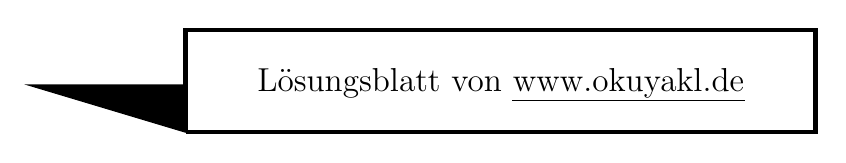
\begin{tikzpicture}(10,3)
	\draw[ultra thick](2,0) --(10,0) -- (10,1.3) --(2,1.3) -- (2,0);
	\draw[fill=black](2,0)-- (0,.6) -- (2,.6) -- (2,0);
	\node at (6,.6) {\large Lösungsblatt von \href{https://www.okuyakl.de}{www.okuyakl.de}};
\end{tikzpicture}
\vspace{0.5 cm}

\noindent {\bf LÖSUNGEN: Aufgabe 1. a)}

Wärme ist die Energie, die zwischen zwei Systemen aufgrund eines Temperaturunterschiedes übertragen wird. Wärme fließt stets vom Ort höherer zum Ort tieferer Temperatur.
\vspace{0.5 cm}

\noindent {\bf Aufgabe 1. b)}

Innere Energie ist die gesamte Energie eines physikalischen Systems, das sich in Ruhe und im thermischen Gleichgewicht befindet. Sie setzt sich z. B. aus der Bewegungsenergie der Teilchen eines Stoffes und ihrer potentiellen Energie zusammen.
\vspace{0.5 cm}

\noindent {\bf Aufgabe 1. c)}

Wasser besitzt seine höchste Dichte bei $\vartheta =\SI{4}{\celsius}$; kühlt man es weiter ab, so dehnt es sich dabei aus. Diese Eigenschaft bezeichnet man als Anomalie des Wassers
\vspace{0.5 cm}

\noindent {\bf Aufgabe 2.}

Erhöht man die innere Energie eines z.B. Feststoffes, 1. so dehnt er sich zunächst aus, 2. kann schmelzen, 3. verdampfen.
\vspace{0.5 cm}

\noindent {\bf Aufgabe 3.}

Er definierte zwei unterschiedliche Temperaturen, den Schmelzpunkt und den Siedepunkt des Wassers, und ordnete ihnen den Wert $\SI{0}{\celsius}$  bzw $\SI{100}{\celsius}$ zu. 
\vspace{0.5 cm}

\noindent {\bf Aufgabe 4.}

Die Teilchen eines Körpers höherer Temperatur bewegen sich stärker als die eines kühleren Körpers. Durch Kontakt zwischen beiden übertragen die schnelleren Teilchen durch Stöße einen Teil ihrer Energie auf die langsameren Teilchen, der Temperaturunterschied wird schließlich ausgeglichen.   
\vspace{0.5 cm}

\noindent {\bf Aufgabe 5.}\\

\begin{minipage}{0.6\textwidth}
Der Heizkörper erwärmt die Luft in seiner Nähe, diese steigt entlang der Wand beim Heizkörper auf bis zur Decke, verteilt sich entlang der Decke und strömt entlang den kühleren Wänden, die keinen Heizkörper haben, wieder herunter und fließt abgekühlt entlang des Bodens wieder dem Heizkörper entgegen. Um die Temperaturunterschiede im Raum gering zu halten, werden Heizkörper bevorzugt an den Stellen mit der stärksten Abkühlung, also unter Fenstern, angebracht.   
\end{minipage}
\hfill
\begin{minipage}{0.35\textwidth}
\includegraphics[width=5cm]{heizung112.pdf}
\end{minipage}
\vspace{0.5 cm}

\noindent {\bf Aufgabe 6.}

\begin{minipage}{0.7\textwidth}
Eine Thermoskanne besteht aus einerem inneren und einem äußeren  Behälter, die durch einen evakuierten Zwischenraum voneinander getrennt sind. Gegen Wärmestrahlung sind die Oberflächen innen verspiegelt. Im Deckel ist eine dicke Isolierschicht aus Kunststoff
\end{minipage}
\hfill
\begin{minipage}{0.25\textwidth}
\includegraphics[width=2.5cm]{thermoskanne112.pdf}
\end{minipage}
\vspace{0.5 cm}

\noindent {\bf Aufgabe 7. a)}

Wärmemenge = Kraft mal Strecke:

$$ \Delta W_{th} = F \cdot d \cdot \pi = \SI{25}{\newton} \cdot \SI{0,056}{\meter} \cdot 3,14 =\SI{4,4}{\joule}$$
\vspace{0.5 cm}

\noindent {\bf Aufgabe 7. b)}

$ W_{th}= \qquad 0,44 \qquad 0,88 \qquad 1,320 \qquad \SI{1,980}{\kilo\joule}$

\begin{minipage}{0.6\textwidth}
\includegraphics[width=5 cm]{diagramm112}
\end{minipage}
\hfill
\begin{minipage}{0.35\textwidth}
Es ergibt sich ein linearer Zusammenhang zwischen der Erwärmung des Zylinders und der zugeführten Energie.
\end{minipage}
\vspace{0.5 cm}

\noindent {\bf Aufgabe 7. c)}

Mit der Formel: 
$$ \Delta  W_{th} = c \cdot m \cdot \Delta \vartheta; \quad \textnormal{also} \quad 
 \Delta  W_{th} \sim \Delta \vartheta $$
ergibt sich ein linearer (=proportionaler) Zusammenhang zwischen den beiden Größen.
Umgestellt ergibt sich für die Masse m mit den Daten aus einem Wertepaar und 
$c_{Messing} =\SI{0,384}{\kilo\joule\over \kilogram\cdot\kelvin}  $:

$$ m = {\Delta  W_{th} \over  c \cdot \Delta \vartheta}=
 {\SI{1,32}{\kilo\joule} \over \SI{0,384}{\kilo\joule\over \kilogram\cdot\kelvin} \cdot \SI{1,5}{\kelvin} } = \SI{2,3}{\kilogram}$$

\begin{center}
	\includegraphics[width=7 cm]{../../viecher/endcomic.pdf}
	
	Hier geht es zurück zum \href{https://www.okuyakl.de/phys/p9thcL112/aa112.pdf}{Aufgabenblatt}
\end{center}

\end{document}